\documentclass[a4paper]{article}
\usepackage[utf8]{inputenc}
\usepackage{multicol}
\usepackage{paracol}
\usepackage{geometry}
\usepackage{amssymb}
\usepackage{graphicx}
\usepackage{wrapfig}
\usepackage{caption}
\usepackage{subcaption}
\usepackage{fancyhdr}
\usepackage[parfill]{parskip}
\usepackage{hyperref}
\usepackage{amsmath}
\usepackage{listings}
\usepackage[table]{xcolor}
\usepackage{mathtools}
\usepackage{array}
\usepackage{enumitem}
\usepackage{wrapfig}
\usepackage{svg}
\usepackage{algorithm2e}
\usepackage[edges]{forest}

% Additional packages permitted by the supplied template.
\usepackage{booktabs}
\usepackage{tabularx}
\usepackage{microtype}
\usepackage{tikz}
\usetikzlibrary{arrows.meta,positioning}

% VS2017 C++ color scheme from the supplied template.
\definecolor{clr-background}{RGB}{255,255,255}
\definecolor{clr-text}{RGB}{0,0,0}
\definecolor{clr-string}{RGB}{163,21,21}
\definecolor{clr-namespace}{RGB}{0,0,0}
\definecolor{clr-preprocessor}{RGB}{128,128,128}
\definecolor{clr-keyword}{RGB}{0,0,255}
\definecolor{clr-type}{RGB}{43,145,175}
\definecolor{clr-variable}{RGB}{0,0,0}
\definecolor{clr-constant}{RGB}{111,0,138}
\definecolor{clr-comment}{RGB}{0,128,0}

\lstset{
    language=Java,
    basicstyle=\ttfamily,
    keywordstyle=\color{blue}\ttfamily,
    stringstyle=\color{red}\ttfamily,
    commentstyle=\color{green}\ttfamily,
    morecomment=[l][\color{magenta}]{\#},
}

\lstset{
    language=Java,
    backgroundcolor=\color{clr-background},
    basicstyle=\color{clr-text},
    stringstyle=\color{clr-string},
    identifierstyle=\color{clr-variable},
    commentstyle=\color{clr-comment},
    keywordstyle=\color{clr-type},
    keywordstyle={[2]\color{clr-constant}},
    tabsize=1,
    frame=single
}

\DeclareMathOperator*{\argmax}{arg\,max}
\DeclareMathOperator*{\argmin}{arg\,min}

\hypersetup{
    colorlinks,
    citecolor=black,
    filecolor=black,
    linkcolor=black,
    urlcolor=black
}

% Geometry is copied unchanged from the official report template.
\geometry{
 a4paper,
 left=18mm,
 right=18mm,
 top=25mm,
 bottom=25mm
}

\graphicspath{{./images/}}
\pagestyle{fancy}
\setlength{\headheight}{14pt}
\fancyhf{}
\fancyhead[L]{Distributed Systems 1 Project}
\fancyhead[R]{Rizzo--Masutti}
\fancyfoot[C]{\thepage}
\raggedbottom
\setlength{\parfillskip}{0pt plus 1fil}

\newcommand{\msg}[1]{\texttt{#1}}
\newcommand{\code}[1]{\texttt{#1}}

\title{\vspace{-20mm}A Quorum-Based Total Order Broadcast Protocol for Distributed Intelligence Databases}
\author{Mattia Rizzo \qquad Alan Masutti}
\date{Distributed Systems 1 Project -- Academic Year 2025--2026}

\begin{document}
    \maketitle
    \section{Project Structure}

\subsection{Objective and execution model}

The system implements a replicated, fixed-length array of integer positions. Clients may contact any replica; reads are answered locally, whereas a distinguished coordinator orders writes. Every client, replica, and emulated point-to-point channel is a Java Akka actor that owns its mutable state and processes one mailbox event at a time. The design assumes static membership, reliable FIFO channels, fail-stop replicas without recovery, accurate bounded failure detection, and a strict majority of correct replicas.

Figure~\ref{fig:architecture} shows the normal request path. An arrow between replicas denotes a dedicated \code{NetworkChannel} actor for that sender--destination pair. The channel queues messages and adds a controlled random delay, but releases the queue head first; therefore latency never reorders messages sent over the same logical channel.

\begin{figure}[h]
\centering
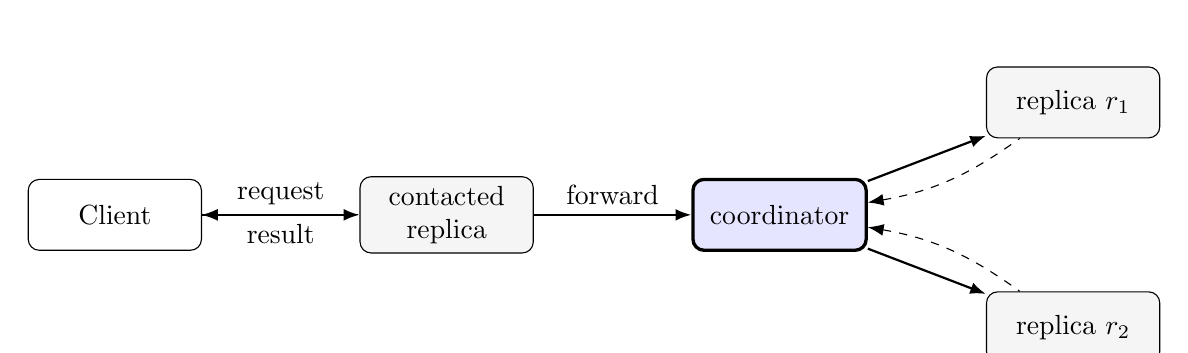
\begin{tikzpicture}[
    node distance=9mm and 20mm,
    actor/.style={draw, rounded corners, minimum width=22mm, minimum height=9mm, align=center},
    coord/.style={actor, fill=blue!10, very thick},
    replica/.style={actor, fill=gray!8},
    channel/.style={-{Latex[length=2mm]}, thick},
    response/.style={{Latex[length=2mm]}-, dashed}
]
\node[actor] (client) {Client};
\node[replica, right=of client] (contact) {contacted\\replica};
\node[coord, right=of contact] (coord) {coordinator};
\node[replica, above right=5mm and 15mm of coord] (r1) {replica $r_1$};
\node[replica, below right=5mm and 15mm of coord] (r2) {replica $r_2$};
\draw[channel] (client) -- node[above]{request} (contact);
\draw[response] (client) -- node[below]{result} (contact);
\draw[channel] (contact) -- node[above]{forward} (coord);
\draw[channel] (coord) -- (r1);
\draw[channel] (coord) -- (r2);
\draw[response] (coord) to[bend right=13] (r1);
\draw[response] (coord) to[bend left=13] (r2);
\end{tikzpicture}
\caption{Normal write path: solid coordinator edges carry UPDATE/WRITEOK; dashed reverse edges carry ACK.}
\label{fig:architecture}
\end{figure}

\subsection{Responsibilities and local state}

\noindent\begin{tabularx}{\textwidth}{@{}>{\bfseries}p{28mm} X X@{}}
\toprule
Component & Responsibility & Principal local state \\
\midrule
\code{Client} & Runs one public read/write operation at a time and reports results or timeouts through callbacks. & Current transaction, FIFO queue, local transaction counter. \\
\code{Replica} & Stores the array, dispatches protocol FSMs, emulates crashes, and records the applied prefix. & $P[0\ldots99]$, coordinator, latest pair, history, active FSMs, crash state. \\
\code{Transaction} & Encapsulates one local READ, WRITE, UPDATE, HEARTBEAT, or ELECTION FSM; it never travels. & Immutable ID and start epoch, FSM state, optional cancellable timeout. \\
\code{NetworkChannel} & Emulates one reliable FIFO link with random latency. & FIFO queue of message/sender pairs and one scheduled delivery. \\
\bottomrule
\end{tabularx}

Protocol messages extend immutable, serializable \code{Msg}. A \code{TransactionId = <initiator, sequence>} correlates a message with one local FSM; it is a routing key, not the database order. The replicated order is the immutable \code{EpochPair} $\langle e,i\rangle$. Heartbeats reserve transaction sequence $0$, ordinary replica FSMs use positive sequences, and elections use negative sequences. The array materializes state for reads; a \code{Map} keyed by \code{EpochPair} records applied transactions. Membership, candidate lists, and synchronization arrays are defensively copied at actor boundaries.

    \clearpage
\section{System Design}

\subsection{Client operations and the normal update protocol}

The client maintains one \code{currentTransaction} and a FIFO queue. A new operation starts only after the previous one returns or reaches its terminal timeout. This is stronger than the required ordering for operations from one client to one replica because it preserves that client's order even when destinations differ.

For a \textbf{read}, \code{ReadTransaction} sends \msg{ReadMsg(idx)} to the selected replica and schedules a local timeout. A live replica validates the index through \code{getPosition}, reads its current array entry, and immediately returns \msg{ReadResultMsg}. The result or the timeout completes the transaction and starts the next queued request.

For a \textbf{write} $w=(idx,val)$, the contacted replica creates a WRITE FSM, which starts the UPDATE FSM below:

\begin{enumerate}[leftmargin=7mm,itemsep=1mm,topsep=1mm]
    \item A non-coordinator forwards $w$ to its known coordinator and waits for \msg{UPDATE}. If the contacted replica is the coordinator, it enters the coordinator path directly.
    \item The coordinator reserves one fresh pair $\langle e,i\rangle$ in mailbox order and broadcasts \msg{UPDATE($\langle e,i\rangle$,idx,val)}. The allocator is separate from the latest applied pair, so an assigned but uncommitted operation is not presented as committed state.
    \item Each receiving replica creates or advances the matching update FSM, returns \msg{ACK($\langle e,i\rangle$)}, and waits for the decision. The coordinator counts itself and waits for
    \[
        |Q|=\left\lfloor\frac{N}{2}\right\rfloor+1.
    \]
    \item On the first quorum, the coordinator broadcasts \msg{WRITEOK} carrying the same non-null pair. A replica applies $P[idx]\leftarrow val$ only after this message, advances its latest pair, stores the update in history, and invokes the required callback.
    \item The trigger replica completes its parent write transaction and returns success to the client. Duplicate or stale acknowledgements cannot create a second decision because the coordinator FSM leaves \code{WAITING\_ACK} after its first quorum.
\end{enumerate}

\subsection{Why all replicas obtain one total order}

Pairs are ordered lexicographically:
\[
\langle e,i\rangle < \langle e',i'\rangle
\iff e<e' \;\lor\; (e=e'\land i<i').
\]
Within an epoch, the coordinator actor reserves pairs and sends UPDATEs in mailbox order. Consider updates $A$ and $B$ with $A$ reserved first. Every participant receives UPDATE $A$ before UPDATE $B$ on its coordinator-to-replica FIFO channel, and sends ACK $A$ before ACK $B$ on its return channel. If $B$ has acknowledgements from a quorum, those same actors have already sent their acknowledgements for $A$; thus $A$ reaches a quorum no later than $B$. The coordinator sends WRITEOK $A$ no later than WRITEOK $B$, and each coordinator-to-replica FIFO channel preserves this order. A replica can temporarily store prefix $[A]$ while another stores $[A,B]$, but it cannot apply $[B,A]$ or $[B]$. This establishes total-order delivery for every completed epoch.

Sequential consistency then follows from two composition rules. First, the client queue preserves program order. Second, a successful write result is emitted only after the contacted replica applies WRITEOK. Therefore, if the same client next reads that replica, the read is sent after application and observes the write or a later value in the same total order. Reads performed concurrently by different clients may see different-length prefixes, which sequential consistency permits; they never force replicas to disagree on the order of writes.

The protocol also satisfies integrity in the normal case: an update is created from a received request, keyed by one transaction ID and one epoch pair, and applied at most once when that FSM accepts the matching WRITEOK. Validity and eventual delivery depend on the stated reliable-channel, bounded-delay, and surviving-quorum assumptions.

\clearpage
\subsection{Timeouts, heartbeat, and crash detection}

Timeouts are self-messages scheduled through the Akka scheduler. Each FSM stores its current \code{Cancellable}; a valid response cancels it. Cancellation alone is insufficient because an expired event may already be in the mailbox, so protocols additionally reject stale events by state or generation.

\noindent\begin{tabularx}{\textwidth}{@{}p{32mm} X X@{}}
\toprule
Detector & Bound used & Reaction \\
\midrule
Client READ/WRITE & Configured public-API deadline & Report timeout and release the next queued client operation. \\
UPDATE phase & $4L$, where $L=maxLatency+\frac{N}{2}maxLatency$ & A trigger missing UPDATE, or a participant missing WRITEOK, starts election for the known coordinator. \\
Heartbeat watchdog & $3\cdot beatInterval+L$ & The follower accepts only the current watchdog generation and requests election once. \\
Election ACK & $2L$ & Mark the unresponsive successor unavailable and retry at the next ring member. \\
\bottomrule
\end{tabularx}

Every coordinator periodically schedules a local \msg{HeartbeatTickMsg}, then broadcasts a network \msg{HeartbeatMsg}. Followers run a watchdog. A \code{watchdogVersion} increments at every reset: if generation $k$ was cancelled after its event entered the mailbox, \msg{WatchdogExpired($k$)} cannot invalidate generation $k+1$. The heartbeat transaction then enters \code{ELECTION\_REQUESTED}, preventing repeated election requests from the same detector.

Three independent observations can expose a failed coordinator: no UPDATE after a forwarded request, no WRITEOK after UPDATE, or no heartbeat. Their expirations need not be simultaneous. To stop these detectors from creating competing coordinators, election initiation is divided into deterministic slots based on ring distance from the failed coordinator. Its immediate correct successor starts first. A later candidate waits for detector skew plus a complete token/ACK ring traversal for every preceding position. In addition, a replica retains at most one preferred election transaction for a failed coordinator and rejects a competing token with a lower priority.

Crash emulation is part of the protocol boundary rather than test-only shared state. A replica has \code{NONE}, \code{PENDING}, and \code{CRASHED} modes. A pending instruction counts a selected category---heartbeat, update, WRITEOK, or election---after each matching send or handled message. Broadcast checks the crash callback after every destination and stops immediately on entering \code{CRASHED}; therefore a test can reproduce partial dissemination rather than only a crash after the whole broadcast. A crashed replica ignores incoming messages and its send helpers return without transmission.

\subsection{Ring election and termination}

Replica IDs sorted increasingly define the logical ring. An \msg{ELECTION} token carries an immutable list of candidates. Each candidate contains its replica ID and latest applied \code{EpochPair}; comparison first selects the greatest pair and then the greatest replica ID to break a tie. This chooses the surviving replica with the longest applied prefix, rather than merely the largest node identifier.

On first receiving the token, a participant appends its snapshot, forwards to the next available ring member, acknowledges the previous sender, and waits for its own successor's ACK. When an ACK times out, \code{RingNavigation} skips that target. Each attempt has an \code{attemptVersion}, so an old ACK timeout cannot skip the target of a newer attempt. If the best candidate becomes unavailable, it is removed and the next-best candidate is tried. Because each timeout permanently adds one failed member to a finite unavailable set, and a strict majority remains correct, forwarding either reaches a correct member or reduces the candidate set; it cannot wait forever on one edge.

\clearpage
\subsection{Synchronization and interrupted updates}

When the token returns to a replica already listed, the participant computes
\[
 winner=\argmax_{r}\bigl(latestPair(r),\; replicaId(r)\bigr).
\]
The winner advances to epoch $1+\max_r epoch(r)$ with baseline pair $\langle e_{new},0\rangle$, records itself as coordinator, and sends every follower a \msg{SYNCHRONIZATION} containing the new identity and a defensive copy of its materialized array. A follower accepts this message only if the announced sender belongs to the static group, matches the announced coordinator, replaces the coordinator it currently considers failed, carries a strictly newer epoch, and has the correct array length.

The full snapshot is intentionally used instead of replaying individual history entries. For a fixed-size array it transfers the same materialized prefix in one immutable message and also repairs a replica that missed several decisions. The winner sends synchronization before recovering waiting writes. Both messages use the same winner-to-follower FIFO channel, so every follower installs the snapshot before seeing a new-epoch UPDATE. The heartbeat FSM is then recreated with the coordinator-scoped ID $\langle coordinator,0\rangle$.

An update timeout records its pre-election phase. If the trigger was still \code{WAITING\_UPDATE}, the failed coordinator never broadcast that request to it, so after synchronization it can safely submit the write to the new coordinator. If it was \code{WAITING\_WRITEOK}, the outcome is uncertain and automatic retry could duplicate an operation already present in the synchronized prefix; that old transaction is therefore cancelled. This is the at-most-once side of recovery.

\subsection{Safety argument and explicit assumptions}

Under the assumptions below, the state of every correct replica is a prefix of a single sequence $S$ of coordinator decisions. Normal operation preserves the prefix invariant by quorum causality and FIFO WRITEOK delivery. Election selects the greatest available prefix, copies it to every correct replica, and starts a greater epoch before accepting further writes. Hence an epoch change cannot reverse two committed updates, and client program order can be embedded in $S$.

The implementation relies on the specification's static unique IDs, reliable FIFO channels, bounded accurate timeouts, fail-stop crashes without recovery, and a strict majority of correct replicas. Client deadlines must cover detection, election, and synchronization; an arbitrarily short external deadline could let a client advance while an earlier outcome is unknown.

There is one additional recovery assumption that must be made explicit. Snapshot election uses the latest \emph{applied} pair, not the set of pending UPDATEs acknowledged before a coordinator crash. Therefore, for an interrupted WRITEOK, at least one correct replica that applied the decision must remain available until synchronization. If the only replicas that applied it all crash before election finishes, the remaining quorum remembers the pending UPDATE but the current election token does not carry it. Removing this stronger assumption would require candidates to include pending quorum evidence (or durable decision records) and the new coordinator to complete that decision before starting its epoch. This limitation does not affect the tested single-coordinator-crash execution, but it is relevant to the specification's strongest uniform-agreement formulation.

    \clearpage
\section{Implementation and Evaluation}

\subsection{State-machine organization}

The implementation separates actor orchestration from per-operation protocol state. \code{Client} and \code{Replica} own and dispatch transactions; each \code{Transaction} implements \code{start()}, \code{computeState(Msg)}, and a small explicit FSM. The arrangement keeps timeout variables and phase-specific data local while allowing a replica to run several updates concurrently.

\noindent\begin{tabularx}{\textwidth}{@{}>{\bfseries}p{29mm} p{43mm} X@{}}
\toprule
FSM & Main states & Terminal event or recovery action \\
\midrule
READ & INIT, WAITING\_RESULT & Result returns the local value; timeout reports failure. \\
WRITE (client) & INIT, WAITING\_RESULT & Result/timeout invokes the supplied client callback and releases the FIFO queue. \\
WRITE (replica) & INIT, WAITING\_UPDATE & Child UPDATE completion sends the result to the originating client. \\
UPDATE & WAITING\_UPDATE, WAITING\_ACK, WAITING\_WRITEOK, WAITING\_ELECTION & Matching WRITEOK applies exactly once; phase timeout starts election; definitely unobserved requests may resume. \\
HEARTBEAT & COORDINATOR, WATCHING, ELECTION\_REQUESTED & Ticks broadcast liveness; a current watchdog expiration requests election. \\
ELECTION & NEW, PARTICIPATING, ELECTED, SYNCHRONIZING & ACK timeout skips a node; winner publishes a snapshot; rejection or synchronization closes old FSMs. \\
\bottomrule
\end{tabularx}

Message dispatch first handles messages that create transactions (READ, WRITE, UPDATE, and ELECTION tokens), then routes subsequent messages by \code{TransactionId}. Replica code iterates over a copy of the active list because a terminal transition may remove its transaction. Results sent to clients use direct actor messaging as public API traffic; all replica-to-replica protocol traffic uses \code{tell}/\code{unicast}/\code{broadcast}, and therefore crosses the emulated FIFO channels.

Two different counters protect different invariants. The transaction counter provides collision-free local routing, while \code{reserveNextUpdateEpochPair()} provides database ordering. The latter is coordinator-only and increments the sequence at reservation time, but \code{Replica.epochPair} changes only when WRITEOK is applied. After synchronization, a changed epoch resets the reservation sequence above the baseline. UPDATE, ACK, WRITEOK, local state, history, and \code{WriteFinishMsg} all carry the same pair; mismatched pairs are ignored and a null pair is rejected where ordering identity is mandatory.

\subsection{Observability and controlled faults}

All required externally visible events use the provided \code{Logger} and callback APIs, so test probes can observe reads, writes, applied updates, election starts, and elected coordinators without shared mutable state. Official logging is timestamped by the template utility; no protocol class prints directly to standard output. Crash instructions are immutable API messages and are interpreted inside the target actor. This makes a failure reproducible at protocol boundaries while preserving normal actor isolation.

The most informative recovery scenario uses five replicas. The coordinator reaches a quorum, sends WRITEOK to one follower, and crashes before completing its broadcast. That follower has pair $\langle0,1\rangle$ while the others remain at $\langle0,0\rangle$. The ring selects the follower with the greater pair, it starts epoch $1$, and synchronization copies value $42$ to all four correct replicas. This case simultaneously exercises partial broadcast, update timeout/heartbeat detection, candidate ordering, election termination, state transfer, and post-election reads.

\clearpage
\subsection{Verification strategy and results}

Verification combines course tests, protocol regressions, formatting, and static analysis. Akka \code{TestKit} listeners receive mandatory callbacks, so tests primarily assert external behavior; focused probes expose identities and history where no callback exists.

\noindent\begin{tabularx}{\textwidth}{@{}>{\bfseries}p{34mm} X p{25mm}@{}}
\toprule
Test layer & Evidence covered & Result \\
\midrule
Course base tests & API shape; initialization; no-crash reads/writes; crash scenarios and callback timing. & Passed \\
Transaction regressions & Message equality/routing; read and write success/timeout; heartbeat generations; update quorum; ring navigation, ACK skipping, candidate choice, synchronization validation. & Passed \\
Consistency regressions & Unique monotonic epoch pairs; six concurrent writes from two clients on five replicas; write-then-read program order; coordinator crash during first WRITEOK followed by convergence. & 4/4 passed \\
Complete JUnit run & All non-contract tests in the repository. & 80/80 passed \\
Quality checks & PMD, SpotBugs, CPD, and Spotless aggregation. & Build successful \\
Remote CI & GitHub \code{Regression CI/run-tests} on the exact implementation head. & Passed \\
\bottomrule
\end{tabularx}

The complete suite was run with an isolated Gradle home because the machine's default Gradle cache could not load its native Linux library. The commands were:

\begin{verbatim}
GRADLE_USER_HOME=/tmp/coredump-gradle-home gradle test --no-daemon
GRADLE_USER_HOME=/tmp/coredump-gradle-home gradle regression --no-daemon
GRADLE_USER_HOME=/tmp/coredump-gradle-home gradle staticAnalysis --no-daemon
\end{verbatim}

Static analysis completed with zero errors and zero formatting findings. Its 42 warnings, two informational findings, and two duplication locations are non-blocking complexity/style observations; correctness instead rests on the stated invariants and fault-oriented tests.

\subsection{Requirement coverage}

\noindent\begin{tabularx}{\textwidth}{@{}p{43mm} X@{}}
\toprule
Required property & Implementation mechanism \\
\midrule
Reliable total-order update delivery & Coordinator pairs, strict-majority ACK, apply-on-WRITEOK, and FIFO channels. \\
Sequential client observations & One active client transaction, FIFO pending queue, and result only after contacted-replica application. \\
Coordinator crash detection & UPDATE/WRITEOK phase deadlines plus versioned heartbeat watchdog. \\
Ring election with crashes & Sorted IDs, immutable candidate token, per-hop ACK timeout, failed-node skipping, and finite candidate reduction. \\
Most up-to-date coordinator & Lexicographic latest-pair comparison with replica-ID tie-break. \\
Post-election convergence & Strictly newer epoch and immutable full-array synchronization before new-epoch traffic. \\
Specific crash points and encapsulation & Per-message crash counters, interruptible broadcast, actor-owned state, and defensive copies. \\
\bottomrule
\end{tabularx}

\subsection{Use of artificial intelligence}

OpenAI Codex was used to assist in code and text generation. The authors reviewed and tested the generated material; responsibility for the design, code, report, and oral explanation remains with the authors.

\subsection{Conclusion}

The project combines quorum broadcast, coordinator-scoped ordering, FIFO transport, and ring election. A local transaction identifier correlates an FSM; the \code{EpochPair} names a replicated decision. Preserving that pair through WRITEOK gives replicas one ordered prefix, and synchronization establishes the next epoch's baseline. The full automated suite passes, with the snapshot-recovery condition stated explicitly above.

\end{document}
